\clearpage
\title{Problem 4.1}
\author{}
\date{}
\maketitle

\section*{Problem Description}
Write a code to find the min/max number from three numbers (Using registers).

\section*{Tools Used}
\begin{itemize}
    \item emu8086 - 8086 Microprocessor Emulator
    \item MacTeX -\LaTeX  compiler.
    \item VS Code with \LaTeX workshop extension as a text editor.
\end{itemize}

\section*{Process}
\subsection*{Code:}

\begin{multicols}{2}{|}
    \begin{minted}[linenos,breaklines,breakanywhere]{nasm}
DATA SEGMENT
    MSG1 DB "The max number is: "
    ANS DB ?, '$'
DATA ENDS 

CODE SEGMENT
    ASSUME CS:CODE, DS DATA

START:
    MOV AX, DATA
    MOV DS, AX
    
    MOV AX, '8'
    MOV BX, '3'
    MOV CX, '6'
    
    CMP AX, BX
    JG CHK1
    
    MOV DX, BX
    JMP NXT1
    
CHK1:
    MOV DX, AX
        
NXT1:
    CMP DX, CX
    JG CHK2
    MOV AX, CX
    JMP NXT2
    
CHK2:
    MOV AX, DX
    
NXT2:
    MOV ANS, AL
    LEA DX, MSG1
    MOV AH, 9
    INT 21H
    MOV AH, 4CH
    INT 21H
    
CODE ENDS
END START
    \end{minted}
\end{multicols}


\subsection*{Output}
\begin{center}
    \centering
    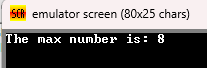
\includegraphics[width = .4\textwidth]{1.png}
    \captionof{figure}{Finding min/max number}
\end{center}

